% !TeX program = xelatex
% 面向数据发布前审查的电力隐性推断源定位方法
% 编译：xelatex（或 tectonic）。版式按南方电网技术投稿模板，正文每页 42 行。
\documentclass[UTF8,zihao=5,twoside]{ctexart}

\usepackage[a4paper,top=22mm,bottom=20mm,left=18mm,right=18mm,%
            headheight=14pt,headsep=6mm,columnsep=7mm,lines=42]{geometry}
\usepackage{fontspec}
\usepackage{xeCJK}
\usepackage{amsmath,amssymb,bm}
\usepackage{graphicx}
\usepackage{float}
\usepackage{booktabs,array,multirow,tabularx}
\usepackage{caption}
\usepackage{titlesec}
\usepackage{fancyhdr}
\usepackage{indentfirst}
\usepackage{enumitem}
\usepackage{multicol}
\usepackage{tikz}
\usetikzlibrary{arrows.meta,positioning,shapes.geometric}
\usepackage[hidelinks]{hyperref}

\graphicspath{{figures/}}

% -------------------- 字体 --------------------
\IfFontExistsTF{Songti SC}
  {\setCJKmainfont{Songti SC}}
  {\IfFontExistsTF{SimSun}
    {\setCJKmainfont{SimSun}}
    {\setCJKmainfont{FandolSong-Regular.otf}[BoldFont=FandolSong-Bold.otf,ItalicFont=FandolKai-Regular.otf]}}
\IfFontExistsTF{Heiti SC}
  {\setCJKsansfont{Heiti SC}}
  {\IfFontExistsTF{SimHei}
    {\setCJKsansfont{SimHei}}
    {\setCJKsansfont{FandolHei-Regular.otf}[BoldFont=FandolHei-Bold.otf]}}
\IfFontExistsTF{Times New Roman}{\setmainfont{Times New Roman}}%
  {\IfFontExistsTF{TeX Gyre Termes}{\setmainfont{TeX Gyre Termes}}{\setmainfont{Latin Modern Roman}}}

\zihao{5}
\setlength{\parindent}{2em}
\linespread{1.08}
\setlist{nosep,leftmargin=2em}
\setlength{\textfloatsep}{0.7em plus 0.2em minus 0.2em}
\setlength{\floatsep}{0.6em plus 0.2em minus 0.2em}
\setlength{\intextsep}{0.6em plus 0.2em minus 0.2em}
\renewcommand{\topfraction}{0.95}
\renewcommand{\bottomfraction}{0.85}
\renewcommand{\textfraction}{0.05}
\renewcommand{\floatpagefraction}{0.85}

% -------------------- 页眉页脚 --------------------
\pagestyle{fancy}
\fancyhf{}
\fancyhead[LE]{\zihao{-5}第~\thepage~页}
\fancyhead[CE]{\zihao{-5}南方电网技术}
\fancyhead[RE]{\zihao{-5}第~XX~卷}
\fancyhead[LO]{\zihao{-5}\thepage}
\fancyhead[CO]{\zihao{-5}南方电网技术}
\fancyhead[RO]{\zihao{-5}第~XX~卷}
\renewcommand{\headrulewidth}{0.4pt}
\renewcommand{\footrulewidth}{0pt}

% -------------------- 标题层级 --------------------
\titleformat{\section}{\sffamily\zihao{4}\bfseries}{\thesection}{0.6em}{}
\titleformat{\subsection}{\sffamily\zihao{5}\bfseries}{\thesubsection}{0.6em}{}
\titlespacing*{\section}{0pt}{0.8em}{0.4em}
\titlespacing*{\subsection}{0pt}{0.6em}{0.3em}

% -------------------- 图表与公式 --------------------
\captionsetup{font={small},labelfont=bf,labelsep=quad,justification=centering}
\renewcommand{\figurename}{图}
\renewcommand{\tablename}{表}
\renewcommand{\theequation}{\arabic{equation}}
\newcommand{\figbicaption}[2]{\caption{#1\\[-0.2em]\small Fig.\,\thefigure\ #2}}
\newcommand{\tabbicaption}[2]{\caption{#1\\[-0.2em]\small Tab.\,\thetable\ #2}}
\renewcommand{\refname}{参考文献}

\newcommand{\articleinfo}{文章编号：1674-0629(20XX)XX-XXXX-XX\quad 中图分类号：TM73\quad 文献标志码：A\\
DOI：10.13648/j.cnki.issn1674-0629.20XX.XX.XXX}

\begin{document}
\twocolumn[

\begin{center}
{\zihao{-5}\articleinfo}\par\vspace{1.0em}
{\sffamily\zihao{2}\bfseries 面向数据发布前审查的电力隐性推断源定位方法}\par\vspace{0.8em}
{\zihao{4}杜浩存}\par\vspace{0.4em}
{\zihao{5}（西安交通大学 网络空间安全学院，陕西 西安 710049）}\par\vspace{0.8em}
\end{center}

\noindent\textbf{摘要：}电网企业在对外发布运行数据前需要判断一批字段能否公开，其难点不在单个字段是否敏感，而在于若干本身不敏感的字段组合后可能反推出不公开的运行细节；候选字段的组合数随字段规模指数增长，逐字段人工对照难以覆盖，且已知公式只能查出显式关系。为此，将发布前审查形式化为可推断性度量问题，提出一种两层剥离与分解式稀疏门控相结合的隐性推断源定位方法。第一层按数据定义枚举分量—汇总关系等已知公式并逐层剥离，把规则可枚举的风险与需要评估的风险分开；第二层在剩余候选上训练分解式稀疏门控深度网络，门控值由多个因子相乘构成并对因子施加二次惩罚，收敛后大部分字段的门控值被精确压至零，选中结果在十余个数量级的阈值范围内保持不变。在美国 PJM 市场真实数据与 RTS-GMLC 交流潮流算例上的实验表明：PJM 上 12 个目标平均使用 28.3\% 的候选字段即可达到全量模型的推断精度（0.8512 对 0.8438）；RTS-GMLC 上以系统级与分区级汇总量推断具名设备运行量，平均使用 18.9\% 的字段达到 0.9743；同预算下本文方法在两个数据集上均优于 STG、LassoNet、XGBoost 等基线；在块状缺失、字段缺失与数据延迟等降级条件下，选中字段子集与全量模型的精度差保持在 0.02 以内。方法可为发布前审查提供风险强度与集中度的量化依据。\par
\noindent\textbf{关键词：}数据发布审查；隐性推断源；稀疏门控；深度神经网络；电力数据安全\par\vspace{0.8em}

\begin{center}
{\bfseries\large Locating Implicit Inference Sources in Power Data for Pre-Release Review}\par\vspace{0.5em}
{DU Haocun}\par\vspace{0.3em}
{\small (School of Cyber Science and Engineering, Xi'an Jiaotong University, Xi'an 710049, China)}\par\vspace{0.5em}
\end{center}

\noindent\textbf{Abstract:} Before releasing operational data, a power utility must decide whether a batch of fields can be published. The difficulty lies not in the sensitivity of individual fields, but in the fact that several individually innocuous fields may jointly reveal non-public operational details. The number of field combinations grows exponentially, so field-by-field manual review cannot provide coverage, and known formulas only reveal explicit relations. This paper formulates pre-release review as an inferability measurement problem and proposes an implicit inference-source localization method combining two-layer stripping with factorized sparse gating. The first layer enumerates known formulas such as component-to-aggregate relations and strips them layer by layer, separating rule-enumerable risk from risk that requires evaluation. The second layer trains a factorized sparse gating network on the remaining candidates, where each gate is a product of factors under quadratic penalty; after convergence most gates are driven exactly to zero and the selected set remains unchanged across more than ten orders of magnitude of the threshold. Experiments on real PJM market data and the RTS-GMLC AC power-flow case show that, for 12 targets on PJM, 28.3\% of candidate fields suffice to match the full model (0.8512 versus 0.8438); on RTS-GMLC, where system- and area-level aggregates are used to infer named device-level quantities, 18.9\% of fields achieve 0.9743. Under an equal field budget the proposed method outperforms STG, LassoNet and XGBoost on both datasets, and under block missingness, field loss and data delay the accuracy gap between the selected subset and the full model stays within 0.02. The method provides a quantitative basis of risk intensity and concentration for pre-release review.\par
\noindent\textbf{Key words:} data release review; implicit inference source; sparse gating; deep neural network; power data security\par\vspace{0.8em}

\noindent{\small 基金项目：无。\\ Foundation item: None.}
\vspace{0.8em}
]

\section{引言}

随着电力数据共享和对外服务的推进，电网企业需要将部分运行与市场数据向科研机构、市场主体或社会公众发布\cite{ref-zhu-sharing,ref-liu-cps}。发布之前必须有人判断：这批字段公开之后，会不会让本不应公开的运行细节被外部还原出来。这项工作在实践中由数据管理部门的审查人员承担，其结论直接决定一批数据能否发布、是否需要在发布前做聚合或降精度处理。

审查的难点不在单个字段。单个字段是否敏感，通常有明确的制度规定可循；真正困难的是\textbf{字段组合}：若干个各自不敏感的公开字段放在一起，可能足以把某个不公开的量还原到很高精度。候选字段常有数十至上百个，其子集数量随字段规模指数增长，逐个组合人工核对并不现实。同时，现行做法主要依赖已知公式与业务定义进行核对，只能发现可以显式写出映射关系的部分，无法发现那些没有公式、却在长期运行中稳定成立的统计依赖。

文献\cite{ref-liu-data-inference}将这类问题归纳为信息物理融合系统中的数据推断威胁，指出低安全等级数据可能通过统计依赖或模型推断恢复高价值目标数据。沿用该范式，本文把可推断性区分为两类。一类是\textbf{公式可算}：目标与若干公开字段之间存在确定映射，例如某具名机组出力被计入其所属燃料类型与所属分区的各级发电汇总量，这类关系写在数据定义中，可以靠规则枚举。另一类是\textbf{隐性推断}：不存在可显式写出的映射，但由于潮流约束、机组组合与市场出清的共同作用，目标与一组公开字段之间形成长期稳定的统计依赖，模型可据此近似还原目标。承载后一类关系的字段集合，本文称为\textbf{隐性推断源}。两类风险的管理方式截然不同：前者可枚举，可以一次性写入发布规范；后者无法写成规则，只能依靠数据评估，且会随运行方式与市场规则变化而改变。

在方法层面，相关性分析\cite{ref-lan-load,ref-szekely-dcorr}计算代价低、结果直观，但只刻画两两依赖，无法判断某字段在多字段联合推断中是否不可替代。本文在 PJM 数据上的实测显示，对净实际交换功率而言，联合模型中最关键的字段按两两相关性仅排在 48 个候选中的第 40 位，六类相关性指标与门控值的秩相关仅为 0.057。稀疏线性模型\cite{ref-tibshirani-lasso}具备变量选择能力但受线性假设限制；树模型重要性排序易受冗余字段和训练随机性影响\cite{ref-chen-xgboost}；全量深度模型只能给出整体可预测性，无法说明哪些字段构成主要推断路径。近年提出的输入端门控方法\cite{ref-yamada-stg,ref-lemhadri-lassonet}可在训练中同时完成拟合与字段选择，但选中字段数往往依赖人工设定的阈值或正则强度。

本文的工作包括三个方面：一是把发布前审查形式化为可推断性度量问题，明确审查需要回答的问题及其可计算形式；二是提出两层剥离流程，把公式可算的风险与需要评估的隐性推断风险分离，直接回答“物理规律与已知公式能算出多少、剩余部分还有多少”；三是采用并适配分解式稀疏门控完成隐性推断源定位，利用其门控值收敛到精确零的性质避免人工设定阈值，并以还原精度与所需字段占比两个维度输出风险分级依据。

\section{问题描述}

\subsection{发布前审查的形式化}

记待发布的候选字段集合为 $F=\{f_1,\dots,f_n\}$，不公开的敏感量集合为 $S=\{s_1,\dots,s_m\}$。对任意子集 $A\subseteq F$，定义敏感量 $s$ 关于 $A$ 的\textbf{可推断性}
\begin{equation}
\rho(s\mid A)=\sup_{g\in\mathcal{G}}\ \mathrm{R}^2\big(s,\ g(A)\big)
\end{equation}
式中 $\mathcal{G}$ 为容量足够的函数类，$\mathrm{R}^2$ 在独立测试集上计算。发布决策即选择 $A\subseteq F$ 使
\begin{equation}
\max_{s\in S}\rho(s\mid A)\le \rho^{\ast}
\end{equation}
其中 $\rho^{\ast}$ 为可接受的还原精度上限。

该形式化直接暴露了审查的困难：决策对象是字段子集而非单个字段，$2^n$ 个子集无法穷举；制度只能规定单个字段是否敏感，无法预先规定任意组合的效果。

\subsection{两类可推断性}

将 $\rho$ 的来源分解为两部分。若存在文档写明的映射 $h$ 使 $s=h(A_0)$ 对某 $A_0\subseteq F$ 成立，则称该部分为公式可算，典型形态包括：分量—汇总关系（$s$ 是某公开汇总量求和中的一项）、会计恒等式（如净交换等于计划交换与非计划交换之差）与乘积关系（如占比等于分量除以总量）。其余部分为隐性推断。

区分两者的意义在于处置方式不同：公式可算部分可枚举、可写入发布规范并长期有效；隐性推断部分只能靠数据评估，需随运行条件变化定期重估。因此本文方法先剥离前者，再度量后者。

\subsection{隐性推断源}

在剥离公式可算关系后的候选池 $\tilde F$ 上，若存在子集 $A^{\ast}\subseteq\tilde F$ 使 $\rho(s\mid A^{\ast})$ 接近 $\rho(s\mid \tilde F)$ 且 $|A^{\ast}|$ 尽可能小，则称 $A^{\ast}$ 为 $s$ 的隐性推断源。

需要说明的是，$A^{\ast}$ 一般不唯一。电力数据中同一信息常由多个字段以不同口径重复携带，因此存在多组规模相近、效果相当的解。本文并不主张“屏蔽 $A^{\ast}$ 即可消除风险”，而是把 $\big(|A^{\ast}|,\ \rho(s\mid A^{\ast})\big)$ 作为风险的\textbf{集中度}与\textbf{强度}度量：前者说明需要多少字段才能完成还原，后者说明还原能达到什么水平。

\section{隐性推断源定位方法}

\subsection{总体流程}

方法流程如图~\ref{fig:flow} 所示，包含三个阶段：已知公式剥离、残差逐层剥离与分解式稀疏门控定位。前两个阶段共同构成“两层剥离”，输出是与公式无关的候选池；第三阶段在该池上定位隐性推断源并给出风险度量。

\begin{figure}[!tbp]
\centering
\begin{tikzpicture}[node distance=3.2mm,
  box/.style={draw,rounded corners=1pt,align=center,inner sep=2pt,
              font=\zihao{-5},minimum width=0.80\columnwidth,minimum height=6.5mm},
  ar/.style={-{Latex[length=1.6mm]},thick}]
\node[box] (a) {候选字段集合 $F$、敏感目标 $s$};
\node[box,below=of a,fill=black!5] (b) {第一层：按数据定义枚举已知公式\\剔除分量--汇总、恒等式、乘积关系};
\node[box,below=of b,fill=black!5] (c) {第二层：按残差逐层剥离\\每层只删贡献最大的一个字段};
\node[box,below=of c] (d) {与公式无关的候选池 $\tilde F$};
\node[box,below=of d,fill=black!10] (e) {分解式稀疏门控网络\\门控值为多因子乘积，因子受二次惩罚};
\node[box,below=of e] (f) {风险度量 $\big(|A^{\ast}|,\ \rho\big)$：集中度与强度};
\foreach \x/\y in {a/b,b/c,c/d,d/e,e/f} \draw[ar] (\x)--(\y);
\end{tikzpicture}
\figbicaption{隐性推断源定位总体流程}{Overall workflow of implicit inference source localization}
\label{fig:flow}
\end{figure}

\subsection{第一层：已知公式剥离}

第一层按数据定义枚举公式，\textbf{不使用任何阈值}，因为依据是官方口径而非数据拟合结果。其中最易被忽略的是分量—汇总关系：若目标 $s$ 本身是某公开汇总量求和中的一项，则该汇总量必须剔除，且要覆盖\textbf{全部汇总层级}。以某具名燃气机组为例，它同时被计入同燃料的全系统汇总、所在分区的同燃料汇总、所在分区的发电总量与系统发电总量，四个层级都需剔除。是否真正造成泄露不影响是否剔除——判据是关系能否由规则枚举，而非其在特定数据上的强弱。

\subsection{第二层：残差逐层剥离}

第一层剥完后，数据中可能仍存在未写入文档、但确定成立的路径。第二层反复执行：在当前候选池上寻找能把目标线性还原到相对残差低于门槛 $\tau$ 的最小支撑集，删去其中贡献最大的一个字段，再重新寻找，直至找不到满足条件的关系。

每层只删一个字段而非整组，是因为整组删除会连带移除可能参与其他路径的字段，导致挖掘深度不足。寻找支撑集采用从全集出发的反向消元而非前向贪心：对形如“边际损耗价等于总电价减能量价格再减阻塞价”的差式关系，目标是两个大数相减所得的小量，只加入其中单个字段时残差反而增大，前向贪心无法到达正确组合。

\subsection{第三层：分解式稀疏门控}

在候选池 $\tilde F$ 上训练带输入门控的深度网络。与在网络参数上做结构化剪枝不同，此处门控作用于\textbf{输入字段}，其取值直接对应字段是否参与推断。本文采用文献\cite{ref-dgating}提出的分解式稀疏门控（factorized sparse gating，FSG）：第 $j$ 个字段的门控值写成 $D-1$ 个因子的乘积
\begin{equation}
g_j=\prod_{d=1}^{D-1}\gamma_{d,j}
\end{equation}
第一层等效权重为 $\bm{\omega}_j g_j$，训练目标为
\begin{equation}
\min\ \mathcal{L}\big(y,\hat y\big)+\lambda\Big(\|\bm{\omega}\|_2^2+\|\bm{\gamma}\|_2^2\Big)
\end{equation}

该形式的关键性质是：对乘积参数化施加二次惩罚，等价于对乘积本身施加 $\ell_{2/(D-1)}$ 惩罚。当 $D-1=2$ 时恰好等价于 $\ell_1$，$D-1>2$ 时稀疏性强于 $\ell_1$。因此门控值收敛后不是趋近于零而是\textbf{精确达到零}，被淘汰字段与保留字段之间出现明显断崖，避免了门控方法中常见的阈值主观性问题。全部因子初始化为 1，训练起点每个字段的门控值均为 1。

由于门控值与第一层权重之间存在尺度不确定性（同时缩放 $g_j$ 与 $\bm{\omega}_j$ 不改变网络输出），每步更新后对第一层权重按列归一化并将其范数并入门控值，以保证门控值可比。

\subsection{风险度量输出}

取门控值不低于活跃阈值的字段构成 $A^{\ast}$，在其上重新训练一个不含门控的普通网络，得到还原精度 $\rho$。以 $\big(|A^{\ast}|/|\tilde F|,\ \rho\big)$ 作为该敏感目标的风险坐标：纵坐标反映风险强度，横坐标反映风险集中度。二者结合可区分“少数字段即可高精度还原”与“需要大量字段联合才能还原”两种情形，为后续处置提供依据。

\section{实验与结果分析}

\subsection{实验设置}

采用两个数据集。

\textbf{PJM 2025 年小时级公开数据}，8\,760 个样本、69 个字段，涵盖负荷、分燃料出力、区域交换、辅助服务与市场价格。选取 12 个具有业务意义的量作为敏感目标。该数据集的优势是完全真实，反映实际市场与调度过程。

\textbf{RTS-GMLC 交流潮流算例}，8\,784 个样本，由官方公开的 2020 年负荷与新能源出力曲线经逐小时机组组合与交流潮流求解生成，全部小时收敛、无缺失。该算例的公开候选为系统级、分区级与分燃料级汇总量共 58 个（其中 12 个全年恒定，实际可用 46 个），敏感目标为具名节点电压相角、具名线路负载率、具名机组出力与投入状态。此处的公开／敏感边界由电网实际发布惯例决定，而非人为指定密级：汇总量确属公开发布内容，设备级运行量确属不公开内容。该算例用于检验“用汇总量推断细粒度运行量”这一与实际关切一致的方向。

模型为三层全连接网络（64--32--16），训练 200 轮，批大小 50，学习率 $1\times10^{-3}$，样本按 8:2 随机划分，随机种子固定。惩罚系数 $\lambda=0.005$，因子数 $D-1=3$，活跃阈值取 0.01。评价指标为独立测试集上的 $\mathrm{R}^2$。所有对比方法使用同一候选池与同一评估流程。

\subsection{公式可算关系的发现与剥离}

表~\ref{tab:strip} 给出 RTS-GMLC 上两层剥离的结果。三类目标呈现出完全不同的形态。

\begin{table}[!tbp]
\centering
\tabbicaption{RTS-GMLC 上的两层剥离结果}{Two-layer stripping results on RTS-GMLC}
\label{tab:strip}
\zihao{-5}
\begin{tabular}{lcccc}
\toprule
目标类别 & 候选起点 & 公式剔除 & 逐层剔除 & 剩余 \\
\midrule
节点电压相角（3 个） & 46 & 0 & 0 & 46 \\
线路负载率（5 个） & 46 & 3 & 0 & 43 \\
机组 121 核电出力 & 46 & 4 & 14 & 28 \\
其余机组量（3 个） & 46 & 4 & 0 & 42 \\
\bottomrule
\end{tabular}
\end{table}

\textbf{节点电压相角两层都未剥除任何字段。} 它不是任何公开汇总量的组成部分，也不存在能把它算出来的近似公式，因此其面临的推断风险全部来自隐性推断。这类字段无法通过核对公式发现风险，只能依靠评估。

\textbf{具名机组出力需要第二层。} 机组 121 为核电机组，第一层剥除其参与求和的四个汇总量之后，线性还原的 $\mathrm{R}^2$ 仍为 1.0000；第二层继续逐层挖掘 14 层，才使残差超过门槛。这说明仅依据已知公式清单并不足以清除确定性路径。

在 PJM 上，12 个目标经第一层剥离后，第二层对总发电量与计量负荷分别再挖 5 层和 6 层，其余目标未发现新的确定性关系。剥离后各目标的线性还原 $\mathrm{R}^2$ 从 0.22 到 0.99 不等，说明剩余的可推断性差异很大，需要逐目标度量。

\subsection{单目标推断源定位与门控演化}

以 PJM 净实际交换功率为例。剥离后候选 48 个，全量模型测试 $\mathrm{R}^2$ 为 0.9673。门控值的演化过程如图~\ref{fig:gate}(a) 所示：训练开始时全部字段的门控值均为 1，随后大部分字段被迅速压低，约 75 轮后已有多数字段落到 $10^{-7}$ 以下并继续趋向精确零；保留下来的字段则稳定在 $10^{-2}$ 以上。

\begin{figure*}[!tbp]
\centering

\includegraphics[width=0.92\textwidth]{fig_gate_evolution.png}
\figbicaption{净实际交换功率的门控值演化与阈值敏感性}{Gate evolution and threshold sensitivity for net actual interchange}
\label{fig:gate}
\end{figure*}

图~\ref{fig:gate}(b) 给出选中字段数随活跃阈值的变化。48 个候选中有 35 个的门控值被精确压至零，其余 13 个非零。因此阈值在 $10^{-13}$ 至 $6\times10^{-3}$ 之间任意取值都得到同样的 13 个字段，跨度超过 10 个数量级；本文取 0.01 时进一步收缩为 11 个。这意味着字段的主要取舍由模型自身完成而非由阈值决定，回应了门控类方法阈值主观性的疑虑。

在选中的 11 个字段上重新训练普通网络，测试 $\mathrm{R}^2$ 为 0.9605，与全量模型的 0.9673 相差 0.0068，而字段数仅为原来的 23\%。作为对照，用未被选中的 37 个字段训练得到 0.8861，明显低于选中子集，说明门控确实识别出了承载主要推断能力的字段。这 11 个字段包括预估小时负荷、总计划交换功率与多类分燃料出力，与交换功率由区域供需差额决定的物理认识一致。

值得注意的是，其中最关键的预估小时负荷按两两相关性在 48 个候选中仅排第 40 位。六类相关性指标与门控值的秩相关系数仅为 0.057。这说明边际相关强度与联合推断中的必要性是两回事：一个字段可能自身与目标关联很弱却不可替代，也可能自身关联很强但信息已被其他字段完全覆盖。因此以两两相关性排序选取字段的做法会遗漏关键字段，联合建模是必要的。

\subsection{多目标与多方法对比}

在两个数据集各 12 个目标上比较六种方法。为保证公平，先由本文方法给出每个目标的字段数 $n$，其余方法按各自的重要性排序取前 $n$ 个，再统一用同一普通网络训练评估。结果如图~\ref{fig:cmp} 所示。

\begin{figure}[!tbp]
\centering
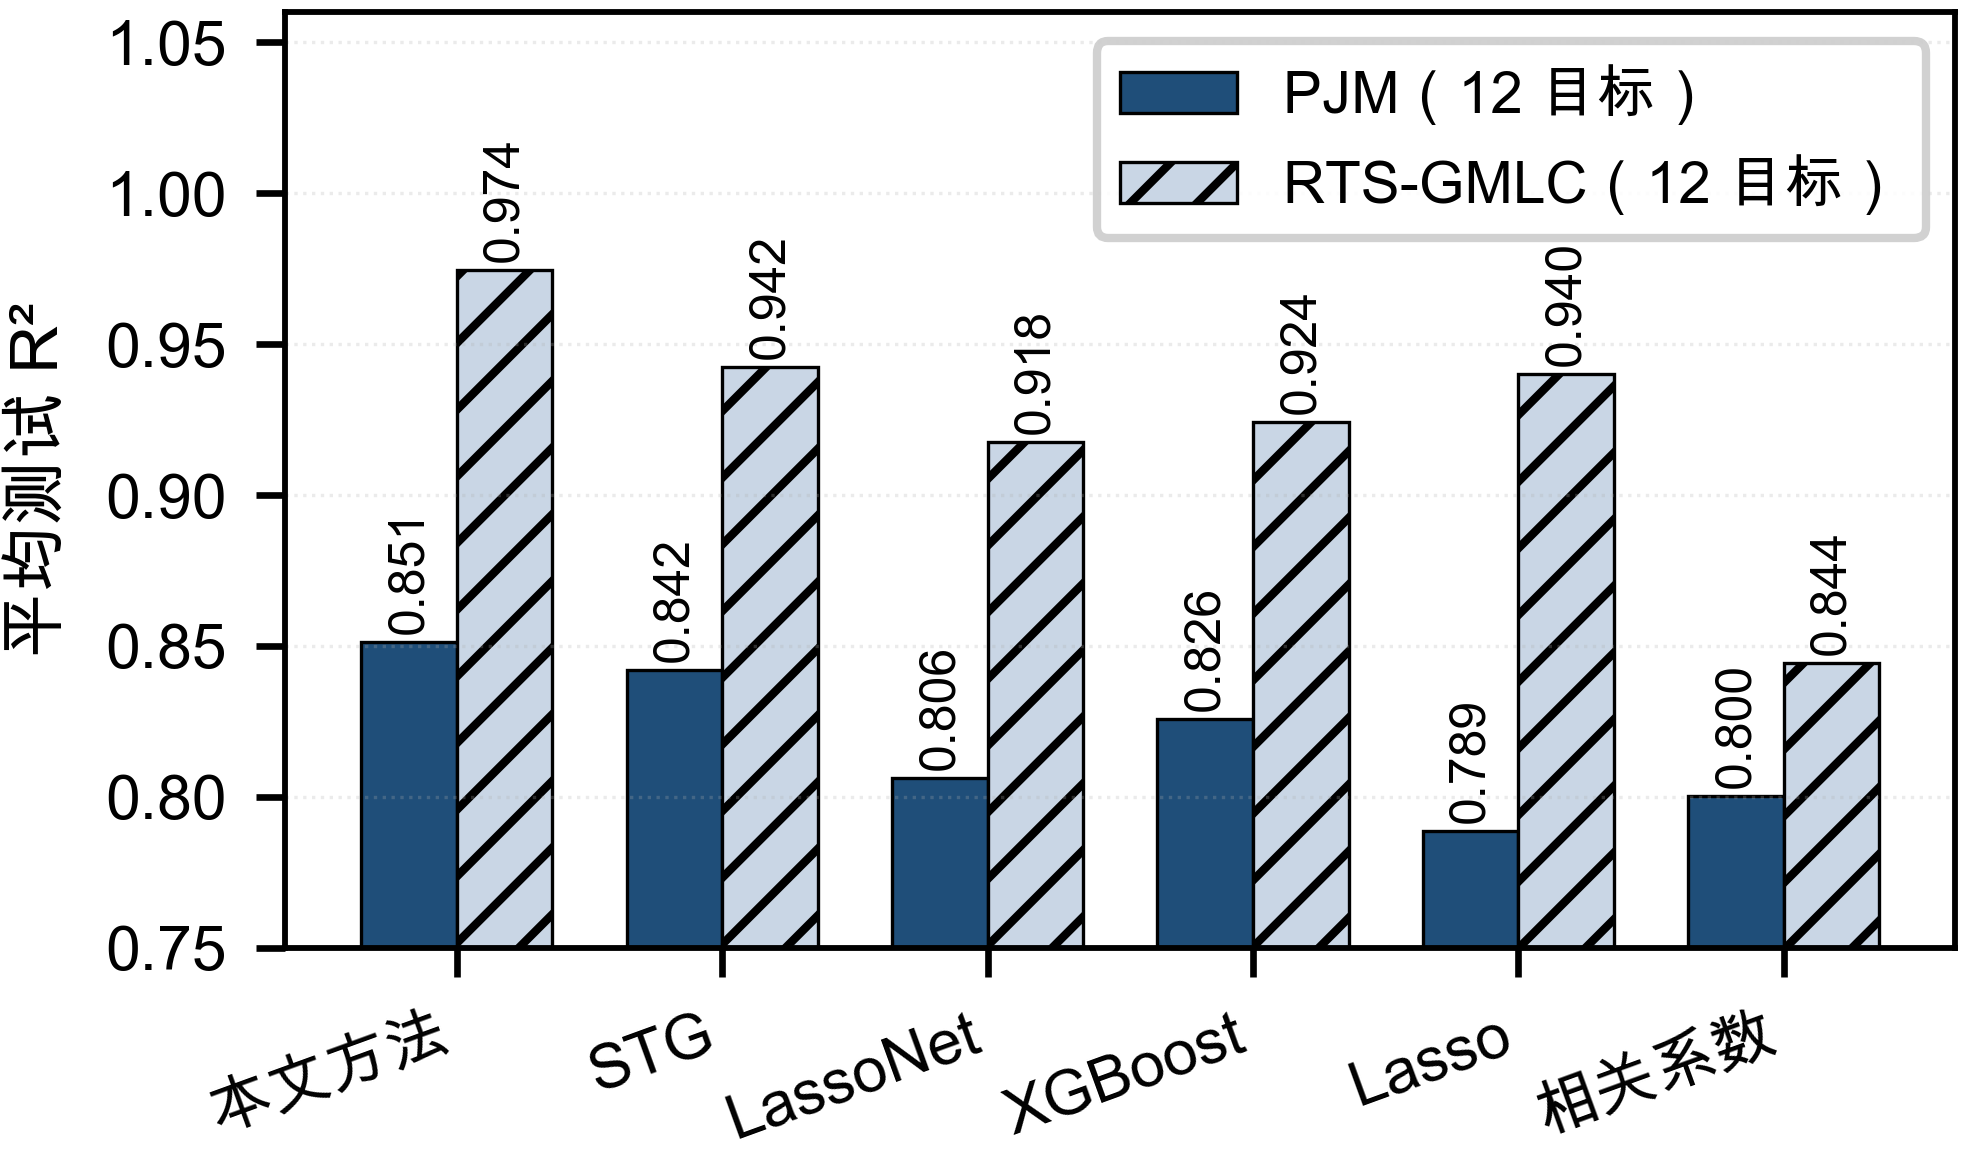
\includegraphics[width=\columnwidth]{fig_method_compare.png}
\figbicaption{同预算下各方法的平均测试 $\mathrm{R}^2$}{Average test $\mathrm{R}^2$ of each method under an equal budget}
\label{fig:cmp}
\end{figure}

本文方法在两个数据集上均排首位：PJM 上 0.8512，次优的 STG 为 0.8420；RTS-GMLC 上 0.9743，次优的 STG 为 0.9423。PJM 上 12 个目标平均使用 13.1 个字段（占候选 28.3\%），选中子集精度 0.8512 略高于全量模型的 0.8438；RTS-GMLC 上平均使用 8.0 个字段（占 18.9\%），选中子集 0.9743 接近全量的 0.9837。选中子集精度可以超过全量模型，是因为剔除无关字段减少了噪声输入。

为检验排名是否依赖于字段数的确定方式，另按原有规则重新确定预算：字段数从 1 开始递增，任一方法首次达到全量模型 95\%（或 97\%）时的字段数作为统一预算。该规则对最先达标的方法有利，结果中如实标出。PJM 上 95\% 与 97\% 两档的统一预算分别为 6.0 与 7.2 个字段，本文方法分别取得 0.8146 与 0.8379，次优方法为 0.7900 与 0.8088；RTS-GMLC 上两档预算为 5.2 与 6.2，本文方法为 0.9348 与 0.9650，次优为 0.9090 与 0.9235。两种预算规则下排名一致，说明领先并非由某一种规则造成。

各目标的风险坐标如图~\ref{fig:risk} 所示。24 个目标中有 12 个落在“少数字段即可高精度还原”的高风险区（还原精度高于 0.9 且所需字段不足候选的 25\%），其中 RTS-GMLC 的具名机组量最为突出：仅用 4 个汇总字段即可将机组出力还原到 0.9989。这类目标即使已剥离全部公式关系，仍可由分区级信息反推，说明发布分区级汇总量时需要格外谨慎。

\begin{figure}[!tbp]
\centering
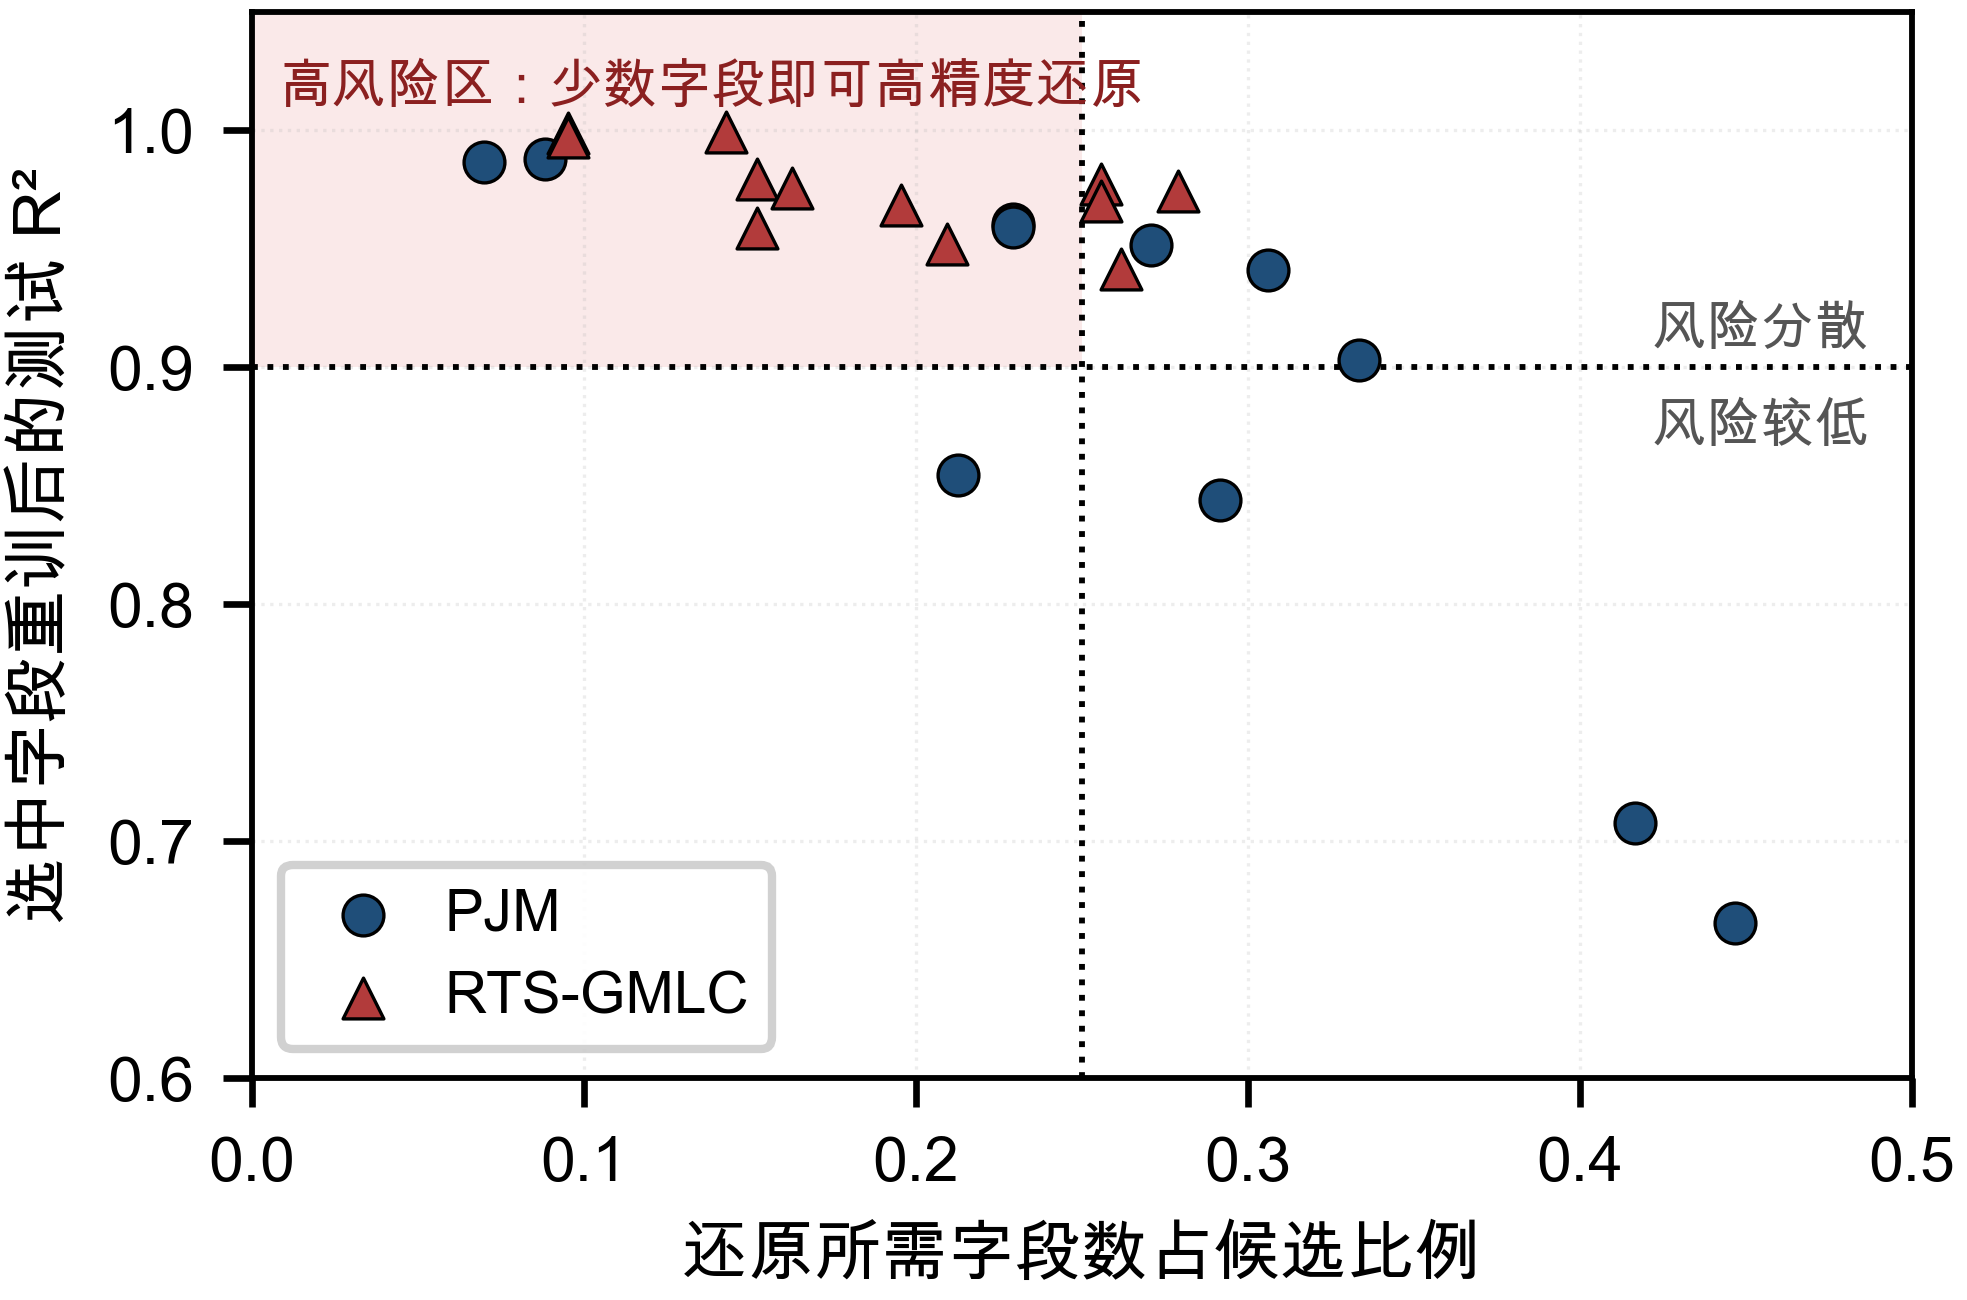
\includegraphics[width=\columnwidth]{fig_risk_map.png}
\figbicaption{各敏感目标的风险坐标}{Risk coordinates of the sensitive targets}
\label{fig:risk}
\end{figure}

\subsection{鲁棒性分析}

实际电网数据常存在缺失、延迟与字段不齐等问题。构造三类降级条件：块状缺失（逐字段随机选取长为 6 小时的时段置为缺失后线性插值，比例 5\%／15\%／30\%）、整字段缺失（随机移除 10\%／20\% 的候选字段）与数据延迟（随机一半字段整体后移 1／3 小时）。缺失按段而非按点构造，以贴近表计掉线、通道中断的实际形态。

在净实际交换功率、日前主用备用总量与日前阻塞价三个目标上的结果如图~\ref{fig:rob} 所示。两项结论如下。

\begin{figure*}[!tbp]
\centering

\includegraphics[width=0.92\textwidth]{fig_robustness.png}
\figbicaption{降级条件下全量模型与选中字段子集的精度}{Accuracy of the full model and the selected subset under degraded conditions}
\label{fig:rob}
\end{figure*}

其一，\textbf{隐性推断本身对数据降级相当稳健}。净实际交换功率在 30\% 块状缺失下全量模型仍达 0.9199，字段缺失 20\% 时为 0.9533，延迟 3 小时时为 0.9516。这一结果的现实含义是：不能指望依靠数据本身的不完善来阻止外部还原。

其二，\textbf{选中字段子集与全量模型的精度基本一致}。全部降级条件下两者之差介于 $-0.022$ 与 $+0.130$ 之间，平均为 $+0.019$；在较难推断的日前阻塞价上，选中子集反而普遍优于全量模型，原因同样是剔除了噪声字段。这说明门控选出的字段集合确实承载了主要推断能力，且该结论在数据不完善时依然成立。

\section{结论}

本文面向电力数据发布前审查场景，把审查工作形式化为可推断性度量问题，提出两层剥离与分解式稀疏门控相结合的隐性推断源定位方法。主要结论如下。

1）将可推断性区分为公式可算与隐性推断两部分是必要的。二者管理方式不同：前者可枚举并写入发布规范，后者只能依靠评估。实验显示节点电压相角这类目标不存在任何可枚举的公式路径，其风险完全来自隐性推断；而具名机组量在剥除四个层级的汇总量后仍需逐层挖掘 14 层才能清除确定性路径。

2）分解式稀疏门控可在无需人工设定阈值的前提下完成字段取舍。门控值收敛后大部分字段被精确压至零，选中结果在超过 10 个数量级的阈值范围内保持不变。PJM 上 12 个目标平均使用 28.3\% 的候选字段达到全量模型精度，RTS-GMLC 上为 18.9\%。同预算下本文方法在两个数据集、两种预算规则下均优于所比较的基线方法。

3）以还原精度与所需字段占比构成的风险坐标可为发布决策提供依据。24 个目标中 12 个落入高风险区，其中具名机组量仅需 4 个汇总字段即可还原至 0.9989。

方法的局限在于隐性推断源一般不唯一：电力数据中同一信息常由多个字段以不同口径重复携带，因此不宜将定位结果理解为唯一的处置清单，而应作为风险强度与集中度的度量。后续工作将围绕多敏感目标之间的耦合关系，以及处置措施代价的量化展开。

\begin{thebibliography}{99}
\zihao{-5}
\bibitem{ref-zhu-sharing}
朱朝阳, 缪思薇, 张宇, 等. 电力数据共享与开放的关键技术研究[J]. 电网技术, 2021, 45(1): 12-21.
\bibitem{ref-liu-cps}
刘烃, 田决, 王稼舟, 等. 信息物理融合系统综合安全威胁与防御研究[J]. 自动化学报, 2019, 45(1): 5-24.
\bibitem{ref-liu-data-inference}
刘烃, 王子骏, 刘杨, 等. 数据推断: 信息物理融合系统数据泄露威胁范式和防御方法[J]. 中国科学: 信息科学, 2023, 53(11): 2152-2179.
\bibitem{ref-lan-load}
兰宇, 王磊, 李明, 等. 基于相关性分析的短期负荷预测特征选择方法[J]. 电力系统保护与控制, 2020, 48(6): 84-91.
\bibitem{ref-szekely-dcorr}
SZ\'{E}KELY G J, RIZZO M L, BAKIROV N K. Measuring and testing dependence by correlation of distances[J]. The Annals of Statistics, 2007, 35(6): 2769-2794.
\bibitem{ref-tibshirani-lasso}
TIBSHIRANI R. Regression shrinkage and selection via the Lasso[J]. Journal of the Royal Statistical Society: Series B, 1996, 58(1): 267-288.
\bibitem{ref-chen-xgboost}
CHEN T, GUESTRIN C. XGBoost: a scalable tree boosting system[C]//Proceedings of the 22nd ACM SIGKDD International Conference on Knowledge Discovery and Data Mining. New York: ACM, 2016: 785-794.
\bibitem{ref-yamada-stg}
YAMADA Y, LINDENBAUM O, NEGAHBAN S, et al. Feature selection using stochastic gates[C]//Proceedings of the 37th International Conference on Machine Learning. 2020: 10648-10659.
\bibitem{ref-lemhadri-lassonet}
LEMHADRI I, RUAN F, ABRAHAM L, et al. LassoNet: a neural network with feature sparsity[J]. Journal of Machine Learning Research, 2021, 22(127): 1-29.
\bibitem{ref-dgating}
Differentiable sparsity via D-Gating: simple and versatile structured penalization[C]//Advances in Neural Information Processing Systems, 2025.
\bibitem{ref-rtsgmlc}
BARROWS C, BLOOM A, EHLEN A, et al. The IEEE reliability test system: a proposed 2019 update[J]. IEEE Transactions on Power Systems, 2020, 35(1): 119-127.
\bibitem{ref-lecun-deep}
LECUN Y, BENGIO Y, HINTON G. Deep learning[J]. Nature, 2015, 521(7553): 436-444.
\end{thebibliography}

\vspace{0.6em}
\noindent{\zihao{-5}\textbf{作者简介：}杜浩存（1999—），男，硕士研究生，主要研究方向为电力数据安全与数据推断分析。}

\end{document}
